%% This is an example first chapter.  You should put chapter/appendix that you
%% write into a separate file, and add a line \include{yourfilename} to
%% main.tex, where `yourfilename.tex' is the name of the chapter/appendix file.
%% You can process specific files by typing their names in at the
%% \files=
%% prompt when you run the file main.tex through LaTeX.
\section{Graphs and disks}
\label{sec:graphs}


\subsection{Graphs}

A graph $G$ is defined as $G = (V,E)$, where $V$ is the set of vertices and $E$ the set of
edges, where $E \subseteq \binom{V}{2}$. The vertices $v,w \in V$ such that $e = vw \in E$
links are called the \textit{endpoints} of $e$.

\begin{defn}
  An embedding of a graph $G$ into a surface $\Sigma$ is a mapping of $G$ in
  $\Sigma$ where the vertices correspond to distinct points and the edges
  correspond to simple arcs connecting the images of their endpoints.
  \cite{goyalGraphEmbeddingTechniques2017}.
\end{defn}

A graph $G$ is planar if there is an embedding of this graph that does not have
any crossing between the edges.

\begin{defn}
  Let $G = (V,E)$ and $S \subset V$, an induced subgraph is a graph $H$ of $G$ whose
  vertex set is $S$ and its edge set $F = \{vw : v,w \in S, vw \in E\}$.
\end{defn}

\begin{defn}
  $H$ is called a \textit{minor} of $G$ if $H$ can be constructed by deleting edges and vertices,
  or contracting edges.
\end{defn}

In graph theory, (forbidden graph characterization)...

\begin{theorem}[Kuratowski]
  A graph $G$ is planar if and only if it doesn't contain $K_5$ or $K_{3,3}$ as a minor or
  a induced subgraph.
\end{theorem}


\subsection{Intersection graphs}

\begin{defn}
The \textit{intersection graph} of a collection $\zeta$ of objects is the graph
$(\zeta,E)$ such that $c_1c_2\in E \Leftrightarrow c_1 \cap c_2 \neq \varnothing$.
\end{defn}


\begin{defn}
  A partial order set is a binary relation $\leq$ over a set $A$ satisfying these axioms:
  \begin{itemize}
    \item $a \leq a$ (reflexivity).
    \item if $a \leq b$ and $b \leq a$ then $a = b$ (antisymmetry).
    \item if $a \leq b$ and $b \leq c$ then $a \leq c$ (transitivity).
  \end{itemize}
\end{defn}

\begin{defn}
   A partially ordered set or poset  $(S,\leq)$ where $S$ a set and $\leq$ a partial
   order on $S$.
\end{defn}

\begin{defn}
  A graph $G$ is a comparibility graph if for each edge $\{u,v\} \in E$ there is
  a binary relation $R$ such that $u \leq v$ or $v \leq u$. Equivalently, $G$
  is a comparability graph if it is the comparability graph of a poset. For
  example, the Hasse diagram (figure \ref{fig:hasse}) is a comparability graph
  where the relation is inclusion.
\end{defn}

\begin{figure}
\centering

\begin{scaletikzpicturetowidth}{\textwidth}
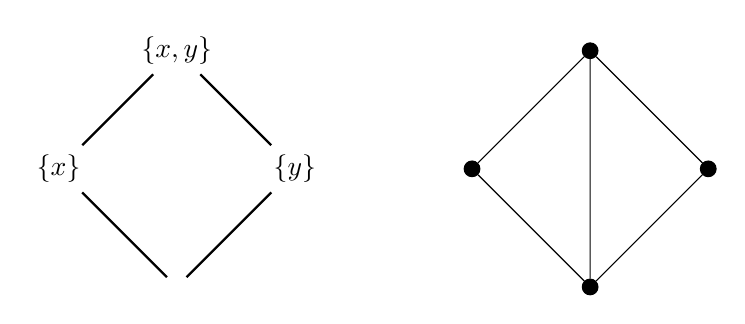
\begin{tikzpicture}[scale=1.5]

  % poset
  \draw (-1cm,0cm) node (v2) {$\{x\}$};
  \draw (1cm,0cm)  node (v3) { $\{y\}$ };
  \draw (0cm,-1cm) node (v4) {$\varnothing$};
  \draw (0cm,1cm)  node (v1) {$\{x,y\}$};

  \draw[thick]  (v1) edge (v2);
  \draw[thick]  (v3) edge (v1);
  \draw[thick]  (v3) edge (v4);
  \draw[thick]  (v2) edge (v4);

  % graph
  \node[draw,circle,inner sep=2pt,fill,label distance=1cm] (v1g) at (3.5,1) {};
  \node[draw,circle,inner sep=2pt,fill,label distance=1cm] (v2g) at (3.5,-1) {};
  \node[draw,circle,inner sep=2pt,fill,label distance=1cm] (v3g) at (4.5,0) {};
  \node[draw,circle,inner sep=2pt,fill,label distance=1cm] (v4g) at (2.5,0) {};
  \draw  (v1g) edge (v2g);
  \draw  (v1g) edge (v4g);
  \draw  (v4g) edge (v2g);
  \draw  (v1g) edge (v3g);
  \draw  (v3g) edge (v2g);

\end{tikzpicture}
\end{scaletikzpicturetowidth}

\caption{On the left, Hasse diagram of a poset of the power set of 2 elements ordered by inclusion.
On the right, the comparability graph of this poset.}
\label{fig:hasse}
\end{figure}

\subsubsection{Interval graphs}

Definition of interval Graphs

Properties

Definition of MIXED interval graphs


\subsection{Realizations}

\begin{defn}
  A graph $G$ is said \textit{realizable} if
\end{defn}

The \textit{graph realizability problem} is the problem that finds a realization
of a given length $l(e)$ for a graph $G$ (this means that the edge $e$ has to
be represented by a straight line of length $l(e)$ in $\mathbb{R}^2$).

A unit distance graph $G$ is a graph that has a realization where 2 points $u,v$
have $\text{dist}(u,v) = 1$ if and only if their respective vertices are adjacent.
This problem  will be shown at chapter \ref{sec:complex} to be $\exists
\mathbb{R}$-complete. If  this realization doesn't have any crossing then $G$ is a
\textit{matchstick graph}.\\

A unit disk graph $G$ is a graph that has a realization where 2 points have
$\text{dist}(u,v) \leq 1$ if and only if their respective vertices are adjacent.
Each point can be represented as the center of a disk of unit diameter and the
edges can be represented as the intersection of 2 disks. This class of graphs
is important for this thesis, as the Thin Strip Graphs are a sub-class of
Unit Disk Graphs (section \ref{sec:thin}). Unit Disk Graph realizability is
$\exists \mathbb{R}$-complete. We will refer to the Unit Disk Graph class as
UDG and an example of a realization can be found in the figure \ref{fig:udg}.

% Figure about the K_1,3 construction
\begin{figure}
\centering

\begin{scaletikzpicturetowidth}{\textwidth}
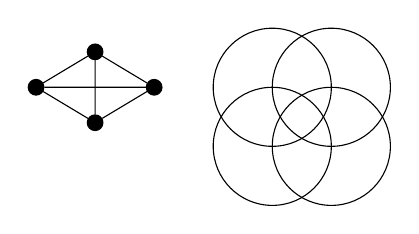
\begin{tikzpicture}[scale=1.5]

  \draw (-0.5,2.5) circle [radius=0.5];
  \draw (0,2.5) circle [radius=0.5];
  \draw (-0.5,2) circle [radius=0.5];
  \draw (0,2) circle [radius=0.5];


  \node[draw,circle,inner sep=2pt,fill,label distance=1cm] (v1) at (-2.5,2.5) {};

  \node[draw,circle,inner sep=2pt,fill,label distance=1cm] (v2) at (-2,2.2) {};
  \node[draw,circle,inner sep=2pt,fill,label distance=1cm] (v3) at (-2,2.8) {};
  \node[draw,circle,inner sep=2pt,fill,label distance=1cm] (v4) at (-1.5,2.5) {};

  \draw  (v3) edge (v2);
  \draw  (v4) edge (v1);
  \draw  (v3) edge (v1);
  \draw  (v4) edge (v2);
  \draw  (v3) edge (v4);
  \draw  (v1) edge (v2);

\end{tikzpicture}
\end{scaletikzpicturetowidth}

\caption{Realization of a UDG (Unit Disk Graph).}
\label{fig:udg}
\end{figure}
